%\documentclass{article}
%\usepackage[utf8]{inputenc}
%\title{test}
%\author{paolo.dini }
%\date{June 2017}
%\begin{document}
%\maketitle
%\section{Introduction}
%\end{document}

%===================================================
%================== DOCUMENT CLASS
%===================================================
\documentclass[runningheads,11pt,a4paper,english,llncs]{Misc/llncs}

%===================================================
%================== PACKAGES
%===================================================
%------------------------------------------------------------------------
% TeX and LaTeX macros
%------------------------------------------------------------------------
%
% In math formulas we use italic instead of mathitalic
%
\makeatletter
% ~ gives a \; space in math mode
\def~{\ifmmode\;\else\penalty\@M\ \fi}
%  Italic in mathematical formulas
\def\@setmcodes#1#2#3{{\count0=#1 \count1=#3
  \loop \global\mathcode\count0=\count1 \ifnum \count0<#2
  \advance\count0 by1 \advance\count1 by1 \repeat}}
\DeclareSymbolFont{italic}{OT1}{\rmdefault}{m}{it}
\let\mathit\undefined
\DeclareSymbolFontAlphabet{\mathit}{italic}
\edef\@tempa{\hexnumber@\symitalic}
\@setmcodes{`A}{`Z}{"7\@tempa41}
\@setmcodes{`a}{`z}{"7\@tempa61}
\makeatother
%
% \begin{asm} ... \end{asm}
%
\newdimen\asmindent     
\asmindent=\parindent
\newcount\asmi
\def\inc{\global\advance\asmi by 1}
\def\dec{\global\advance\asmi by-1}
\def\nl{{}$\par\hangindent\asmi em
  \noindent\kern\asmi em\ignorespaces$} 
\def\asmskip{{}$\par\smallskip\hangindent\asmi em
  \noindent\kern\asmi em\ignorespaces$} 
\def\asm{\global\asmi=0 
%%%%%%%%%%%%%% added by Paolo:
\parskip=0pt
%%%%%%%%%%%%%%%%%%%%%%%
 \def\+{\inc\nl}
 \def\-{\dec\nl}
 \def\\{\nl}
 \begin{trivlist}\item[]\leftskip=\asmindent\relax$}
\def\endasm{$\end{trivlist}}
%\mathindent=\asmindent
%
% \begin{asmarray}
%    f(s_1) & := t_1 \\
%    f(s_2) & := t_2 
% \end{asmarray}
%
\def\asmarray{\begin{array}[t]{@{}l@{\;}l@{\;}l@{}}}
\def\endasmarray{\end{array}}
%
%
%
\def\asmcomment#1{\quad\hbox{// #1}}
%
%  \begin{subasm} ... \end{subasm}
%
\newcount\asmii
\def\subasm{\vtop\bgroup\asmii=0\normalbaselines
 \def\nl##1{$\egroup\advance\asmii by##1\relax\hbox\bgroup\hskip\asmii em$}
 \def\\{\nl{0}}
 \def\+{\nl{1}}
 \def\-{\nl{-1}}
 \hbox\bgroup\hskip\asmii em$}
\def\endsubasm{$\egroup\egroup}
%
% Keywords in ASM code
%
\def\ASM#1{\hbox{\sc#1}}        % rule names and macros
\def\ASMIND#1{\ASM{#1}\index{#1@{\sc#1}}}
\def\AWAIT   {\mathrel{\mathbf{await}}}
\def\AND     {\mathrel{\mathbf{and}}}
\def\CASE    {\mathrel{\mathbf{case}}}
\def\CHOOSE  {\mathrel{\mathbf{choose}}}
\def\CREATE  {\mathrel{\mathbf{create}}}
\def\NEW  {\mathrel{\mathbf{new}}}
\def\DO      {\mathrel{\mathbf{do}}}
\def\ELSE    {\mathrel{\mathbf{else}}}
\def\ELSEIF  {\mathrel{\mathbf{elseif}}}
\def\FORALL  {\mathrel{\mathbf{forall}}}
\def\FORSOME  {\mathrel{\mathbf{forsome}}}
\def\FOREACH  {\mathrel{\mathbf{foreach}}}
\def\FROM  {\mathrel{\mathbf{from}}}
\def\THEREISNO  {\mathrel{\mathbf{thereisno}}}
\def\IF      {\mathrel{\mathbf{if}}}
\def\IFF      {\mathrel{\mathbf{iff}}}
\def\IMPORT  {\mathrel{\mathbf{import}}}
\def\IN      {\mathrel{\mathbf{in}}}
\def\LET     {\mathrel{\mathbf{let}}}
\def\SELF    {\mathrel{\mathbf{self}}}
\def\MATCH    {\mathrel{\textbf{match}}}
\def\NOT     {\mathrel{\mathbf{not}}}
\def\OF      {\mathrel{\mathbf{of}}}
\def\OR      {\mathrel{\mathbf{or}}}
\def\PAR     {\mathrel{\mathbf{par}}}
\def\SEQ     {\mathrel{\mathbf{seq}}}
\def\SKIP    {\mathrel{\mathbf{skip}}}
\def\THEN    {\mathrel{\mathbf{then}}}
\def\TO  {\mathrel{\mathbf{to}}}
\def\WHERE   {\mathrel{\mathbf{where}}}
\def\WHILE   {\mathrel{\mathbf{while}}}
\def\UNDEF   {\mathrel{\mathbf{undef}}}
\def\UNTIL   {\mathrel{\mathbf{until}}}
\def\WHEN   {\mathrel{\mathbf{when}}}
\def\WITH    {\mathrel{\mathbf{with}}}
\def\STEP    {\mathrel{\mathbf{step}}}
\def\STEPWISE    {\mathrel{\mathbf{stepwise}}}
\def\SEQ    {\mathrel{\mathbf{seq}}}
\def\RESULT  {\mathrel{\mathbf{result}}}
\def\CALL  {\mathrel{\mathbf{Call}}}
\def\LOCAL    {\mathrel{\mathbf{local}}}
\def\ADDGUARD {\mathrel{\mathbf{addGuard}}}
\def\ADDUPD   {\mathrel{\mathbf{addUpd}}}
\def\ADDRULE  {\mathrel{\mathbf{addRule}}}
\def\MINUSRULE  {\mathrel{\mathbf{minusRule}}}
\def\TO      {\mathrel{\mathbf{to}}}
%
% Including figures
%
\def\includefig#1#2{\centering\medskip
  \includegraphics[scale=#1]{fig/#2}
  \medskip}
%
% References to paragraphs in the ECMA standard for C#
%
\def\ecma#1{\cite[\S#1]{ecma334}}
%
%  Environments for definitions and theorems
%
%\theorembodyfont{\rm}
%\newtheorem{definition}[subsection]{Definition}
%\newtheorem{lemma}[subsection]{Lemma}
%\newtheorem{theorem}[subsection]{Theorem}
%\newtheorem{proposition}[subsection]{Proposition}
%\newtheorem{corollary}[subsection]{Corollary}
%\newtheorem{example}[subsection]{Example}
%\newtheorem{remark}[subsection]{Remark}
%\newtheorem{constraint}[subsection]{Constraint}
\def\proof{\trivlist\item[]{\bf Proof.}}
\def\endproof{$\Box$\endtrivlist}
%
% enumerate and itemize (smaller skips) from "latex.ltx"
%
\makeatletter
\def\enumerate{%
  \ifnum \@enumdepth >\thr@@\@toodeep\else
    \advance\@enumdepth\@ne
    \edef\@enumctr{enum\romannumeral\the\@enumdepth}%
      \expandafter
      \list
        \csname label\@enumctr\endcsname
        {\usecounter\@enumctr\def\makelabel##1{\hss\llap{##1}}
         \itemsep 0pt\parskip 0pt\parsep 0pt\topsep\smallskipamount}%
  \fi}
\def\itemize{%
  \ifnum \@itemdepth >\thr@@\@toodeep\else
    \advance\@itemdepth\@ne
    \edef\@itemitem{labelitem\romannumeral\the\@itemdepth}%
    \expandafter
    \list
      \csname\@itemitem\endcsname
      {\def\makelabel##1{\hss\llap{##1}}
       \itemsep 0pt\parskip 0pt\parsep 0pt\topsep\smallskipamount}%
  \fi}
\makeatother
%
% items in itemize
%
\def\bull{\vrule height .9ex width .8ex depth -.1ex}
\def\labelitemi{\bull}
%
%
%
\def\cs#1{C\#$_{\mathcal{#1}}$}
\def\lang#1{L$_{\mathcal{#1}}$}
%
% Positions
%
\def\pos#1{{}^{#1}}
\def\termPos{\blacktriangleright}
\def\cursor{\pos{\termPos}}
%
%
%
\def\sup{\hbox{sup}}
\def\c#1{\texttt{#1}}           % code
\def\N#1{\textit{#1}}           % non terminal symbols
\def\T#1{\hbox{`\texttt{#1}'}}  % terminal symbols
\def\A#1{\hbox{\sc#1}}          % ASM rules
\def\D#1{#1}                    % dynamic functions
\def\U#1{#1}                    % universes
\def\C#1{#1}                    % constructors
\def\rdef{\equiv}
\def\lbr{\c{\char`\{}}
\def\rbr{\c{\char`\}}}
\def\mb{\hbox{::}}
\def\map#1#2{\textbf{Map from}~#1~\textbf{to}~#2}
\def\cat{\cdot}
\def\adots{\mathinner{\ldotp\ldotp}}
%
%
% macros.tex ends here
\usepackage{etex}
\reserveinserts{28}
\newcommand{\todo}[1]{
 \noindent{\newline \color{red}
 \framebox[\textwidth][t]{%
  \parbox[t]{0.9\textwidth}{\textcolor{red}{TODO: #1}}                                                                                     
}}}
\usepackage{graphicx}
\usepackage{acronym}
\usepackage{ifthen}
\usepackage{substr}
\usepackage{color}
\usepackage{fixltx2e}
\usepackage[left=2cm, top=2cm, right=2cm, bottom=2cm]{geometry}
%\usepackage{subfigure}
\usepackage{array}  
\usepackage[figuresright]{rotating}          
\usepackage{url}
%\usepackage{enumerate}
\usepackage[shortlabels]{enumitem}
\usepackage{epsfig}
\usepackage{colordvi}
\usepackage{makeidx}
\usepackage{index}
\usepackage[absolute]{textpos}
\setlength{\TPHorizModule}{\paperwidth}
\setlength{\TPVertModule}{\TPHorizModule}
\textblockorigin{-6mm}{0mm}
\usepackage[%
      breaklinks=true,%
      colorlinks=true,%           no frame around URL
      urlcolor=LINK_COLOR,%            no colors
      menucolor=LINK_COLOR,%           no colors
      linkcolor=LINK_COLOR,%           no colors
      pagecolor=LINK_COLOR,%           no colors
      bookmarks=true,%            tree-like TOC
      bookmarksopen=false,%       expanded when starting
      hyperfootnotes=true,%       no referencing of footnotes, does not compile
      citecolor=CITE_COLOR,%           black cites
      filecolor=black,%           black files%
      hyperindex=true,%
      hyperfigures=true%
]{hyperref}
\usepackage{bookmark}
\usepackage{booktabs}
\usepackage{dsfont}
\usepackage{wallpaper}
\usepackage{mathtools,cancel}
\usepackage{soul}
\usepackage{float}
\usepackage{setspace}
%\usepackage{morefloats}
%\usepackage{mdwlist}
\usepackage{amsmath,amssymb,amscd,diagrams,bm,amsfonts}
\let\proof\relax
\let\endproof\relax
\usepackage{amsthm}
%\usepackage{ntheorem}
\usepackage{tabularx, graphics, longtable}
%TIKZ
\usepackage{tikz}
\usepackage{tikz-cd}
\usetikzlibrary{trees,snakes}
\usetikzlibrary{arrows,automata}
\usetikzlibrary{matrix,arrows,positioning}
\usetikzlibrary{mindmap,backgrounds}
\usetikzlibrary{shapes}
\usepackage{verbatim} %for comment out some texts


%%%%%%%%%%%%%%%%%%%%%%%%%%%%%%%
%%%%%%%%%%%%%%%%%%%%% Egon's commands:
\usepackage{latexsym}
\ifx\pdfoutput\undefined
  \message{We are running LaTeX.} 
%PD  \usepackage[dvips]{graphicx}
%PD  \DeclareGraphicsExtensions{.eps}
%PD  \usepackage[hypertex,bookmarks=false]{hyperref}
\else
  \message{We are running PDFLaTeX.}
%PD  \usepackage[pdftex]{color}
%PD  \usepackage[pdftex]{graphicx}
%PD\DeclareGraphicsExtensions{.jpg,.pdf}
%PD  \DeclareGraphicsExtensions{.pdf}
%PD  \usepackage[pdftex,bookmarks=false]{hyperref}
%PD  \hypersetup{colorlinks={true},
%PD            linkcolor={blue},
%PD            citecolor={blue},
%PD            urlcolor={blue},
%PD            plainpages={false}
%PD  }
\fi
%%%%%%%%%%%%%%%%%%%%%%%%%%%%%%%
%%%%%%%%%%%%%%%%%%%%%%%%%%%%%%%

%===================================================
%================== THEOREMS
%===================================================
\theoremstyle{plain}
\newtheorem{thm}{Theorem}
\newtheorem{cor}[thm]{Corollary}
\newtheorem{lem}[thm]{Lemma}
\newtheorem{prop}[thm]{Proposition}
\newtheorem{defin}[thm]{Definition}
\newtheorem{rmrk}[thm]{Remark}

\allowdisplaybreaks

%\newtheorem{case}{Case}
%\theorempostwork{\setcounter{case}{0}}

%===================================================
%================== COLOURS
%==================================================

\definecolor{green}{rgb}{0,0.6,0} 
\definecolor{gray}{rgb}{0.6,0.6,0.6} 
\definecolor{red}{rgb}{1,0,0} 
\definecolor{blue}{rgb}{0,0,1} 
\definecolor{purple}{rgb}{0.5,0,0.5} 
\definecolor{yellow}{rgb}{0.25,0.25,0} 
\definecolor{turquoise}{rgb}{0,0.5,0.5}
\definecolor{brown}{rgb}{0.6,0.2,0.1}

\definecolor{LINK_COLOR}{rgb}{0,0,0.7}
\definecolor{CITE_COLOR}{rgb}{0,0.5,0}
\definecolor{lightblue}{rgb}{0,0,1}
\definecolor{light-gray}{gray}{0.95}
\def\red#1{\textcolor[rgb]{1.0,0.0,0.0}{#1}}
\def\green#1{\textcolor[rgb]{0.0,0.8,0.1}{#1}}
\def\blue#1{\textcolor[rgb]{0.0,0.0,1.0}{#1}}

%===================================================
%================== LAYOUT
%===================================================
\parindent=0cm
%\setlength{\parskip}{1.0\baselineskip plus 0.5ex minus 0.2ex}
\abovecaptionskip=0cm
\hyphenpenalty=5000
\tolerance=1000 
\floatsep=1in
\allowdisplaybreaks
\def \constzeroindent {0cm}
\def \constfirstindent {0.5cm}
\def \constsecondindent {1cm}
\newenvironment{mycustomindent}[1]
{\setlength{\parindent}{#1}}
{\setlength{\parindent}{\constzeroindent}}
\newcommand{
	\firstindent}[1]{
	\begin{mycustomindent}{\constfirstindent}
	\begin{tabular}{@{}p{12cm}@{}}
	#1 \\
	\end{tabular}
	\end{mycustomindent}
}
\newcommand{
	\secondindent}[1]{
	\begin{mycustomindent}{\constsecondindent}
	\begin{tabular}{@{}p{12cm}@{}}
	#1 \\
	\end{tabular}
	\end{mycustomindent}
}
\newenvironment{packed_item1}{
\begin{itemize}[topsep=0pt, partopsep=0pt]
  \setlength{\itemsep}{5pt}
  \setlength{\parskip}{0pt}
  \setlength{\parsep}{0pt}
}{\end{itemize}}
\newenvironment{packed_item2}{
\begin{itemize}[topsep=0pt, partopsep=0pt]
  \setlength{\itemsep}{0pt}
  \setlength{\parskip}{0pt}
  \setlength{\parsep}{0pt}
}{\end{itemize}}
\newenvironment{packed_enumerate}{
\begin{enumerate}[topsep=0pt, partopsep=0pt]
  \setlength{\itemsep}{5pt}
  \setlength{\parskip}{0pt}
  \setlength{\parsep}{0pt}
}{\end{enumerate}}
% The following commands are to get rid of the extra space around section and subsection titles:
% Save the class definition of \subparagraph:
\let\llncssubparagraph\subparagraph
% Provide a definition to \subparagraph to keep titlesec happy:
\let\subparagraph\paragraph
\usepackage[compact]{titlesec}
\usepackage{dblfloatfix,caption,subcaption}
\titlespacing{\section}{0pt}{12pt}{*0}
\titlespacing{\subsection}{0pt}{6pt}{0pt}
\titlespacing{\subsubsection}{0pt}{6pt}{0pt}
% Force section numbering to follow chapter numbering:
\usepackage{chngcntr}
\counterwithin{section}{chapter}
\counterwithin{figure}{chapter}
%\counterwithin{theorem}{chapter}
%\counterwithin{lemma}{chapter}
%\counterwithin{definition}{chapter}
%%%%%%%%%%%%%%%%%%%%%%%%%%%%
% Allow line breaks in long list of citations that would extend into the margin:
\usepackage{breakcites}
%%%%%%%%%%%%%%%%%%%%%%%%%%%%%%%%%%%%%%

\usepackage{pdfpages}
\pagestyle{headings}

\renewcommand{\rightmark}{INTERLACE Project (Grant no.~754494)}
\renewcommand{\leftmark}{D2.3}
\setcounter{tocdepth}{2}

\usepackage{tocloft}
\setlength\cftparskip{0pt}
\setlength\cftbeforechapskip{12pt}

\usepackage{abstract}
\renewcommand{\abstractnamefont}{\large \bfseries}
%\setlength{\abstitleskip}{-\absparindent}
\renewcommand{\abstractname}{Abstract}

\setlength{\parskip}{12pt}

\begin{document}
%===================================================
%================== TITLE
%===================================================

\thispagestyle{empty}
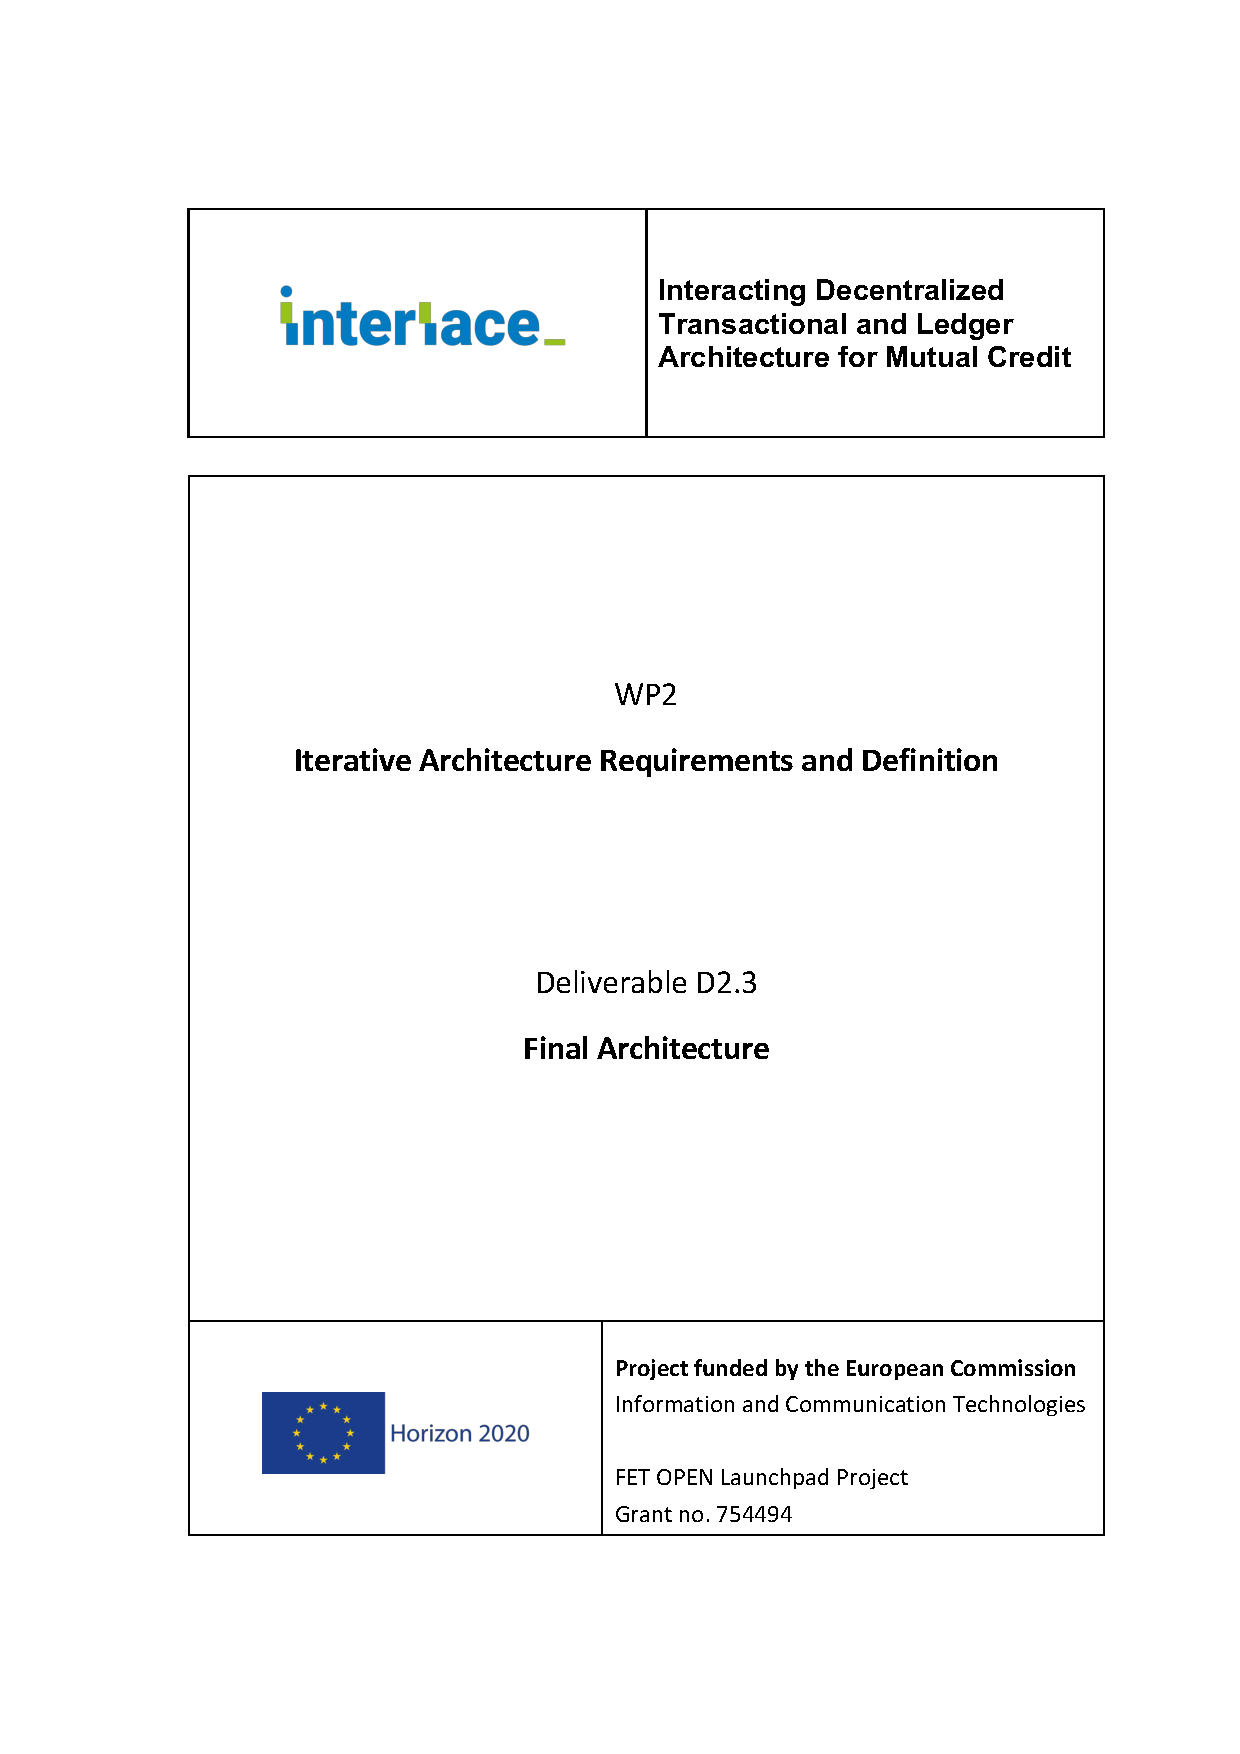
\includepdf[pages=-, scale=1.0]{Misc/Front}

%===================================================
%================== ABSTRACT
%===================================================
\thispagestyle{empty}

\begin{abstract}
\normalsize


\end{abstract}

\newpage

%===================================================
%================== TABLE OF CONTENTS
%===================================================
\tableofcontents

%===================================================
%================== CHAPTERS
%===================================================
\chapter{Introduction}
\label{ch:Introduction}

\vspace{-1cm}
\begin{center}
Paolo Dini and Giuseppe Littera
\end{center}















\newpage












\chapter{Final Architecture}
\label{ch:finarch}

\vspace{-1cm}
\begin{center}
Paolo Dini, Giuseppe Littera, Eduard Hirsch, Luca Carboni, and Aurelio Riccioli
\end{center}

The technical architecture of the system implemented is discussed in some detail in deliverable D3.2 \cite{INTERLACE_D32}. Here we present just the high-level CTO model, which is somewhat analogous to a class diagram. We then present the high-level view of the microservice-based Sardex application architecture; and finally we discuss the long-term view of a global multi-layer open shared architecture within which the Sardex system becomes one of many possible applications.

\section{CTO-Model of the System Implemented}
\label{sec:cto-model}

The CTO-model is specific to the Hyperledger Composer framework and offers the possibility to set-up a ground model which drives the chaincode implementation. `CTO' refers to the initial name of the language used to specify the model, `Concerto'. Even though it was then changed to Go, the extension `.cto' remained. The primitive concepts of a .cto model are:
\begin{quote}
\begin{packed_item1}
\item Transactions
\item Assets
\item Participants
\item Concepts
\item Events
\item Enum
\end{packed_item1}
\end{quote}

As can be seen in Figure \ref{fig:DCN-cto}, the model created for the INTERLACE project has two main \textit{transactions}, \textit{CreditTransfer} and \textit{DebitTransfer}, that inherit from \textit{Transfer}. \textit{DebitTansfer} actually also needs a second transaction named \textit{DebitTransferAcknowledge} to be performed, thus it may be counted as a main transaction as well. Two other transactions supporting the functionality of the network are \textit{InitBlockchain} and \textit{CleanupPendingTransfer}.

Transfers create and update \textit{assets}. When the main transfers are executed they change \textit{Account} assets: namely, \textit{SysAccount} and \textit{MemberAccount} which inherit from \textit{Account}. \textit{DebitTransfer} also needs the \textit{PendingTransfer} asset for creating transfers that have not been confirmed yet. \textit{DeltaDebt} collects all transfers which caused a balance to go negative or that caused a negative balance to go more negative, to log when the debt has to be paid back. Please see the Appendix \ref{appendix} for more details.

In order to perform credit or debit operations a \textit{participant} needs to be registered. There are two participants derived from \textit{Member}, called \textit{Subscriber} and \textit{Individual}. These members may own an account asset which can be used to transfer credits from one account to another.

On several occasions events are emitted which may be consumed by an application or a user to react to specific issues that have happened during a transaction. There are several different events that may be of interest to a user, but for the moment only three are implemented: \textit{LimitViolation} warns of a possible account limit violation; \textit{RequestDebitAcknowledge} asks a user to give an acknowledgement to a pending transaction; and \textit{DebitAcknowledgeInvalid} informs the user that the acknowledgement for a pending transaction was denied or is invalid.


\begin{figure}[h]
\centering
\frame{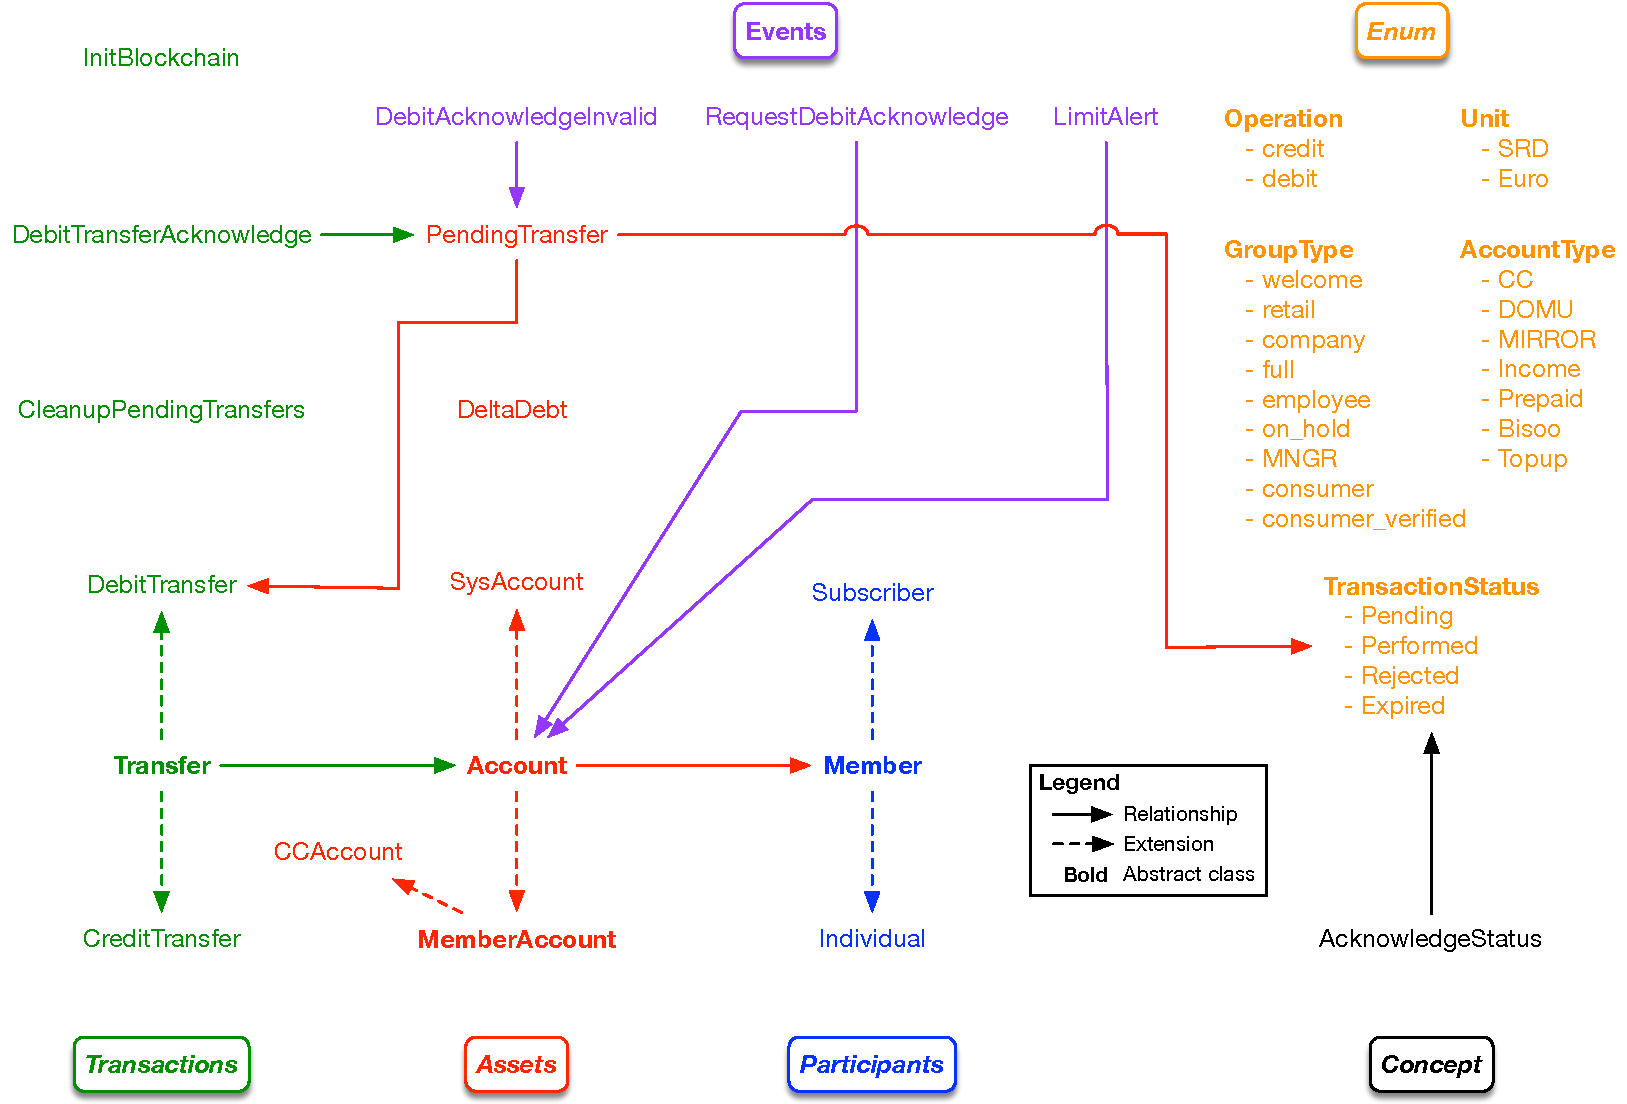
\includegraphics[width=16 cm]{Figures/DCN}}
\caption{\bf \small Hyperledger .cto model/class diagram of INTERLACE transactional platform}
\label{fig:DCN-cto}
\end{figure}


Finally, there are a few \textit{enum} types with states names for operations and units as well as account and group types. A detailed explanation of the model language can be found the official hyperledger composer documentation\footnote{\url{https://hyperledger.github.io/composer/latest/reference/cto_language.html}}

\section{Sardex Application Architecture}
Figure \ref{fig:HL_Architecture} provides a snapshot of the high-level application architecture of the Sardex system. The detailed Legend of the figure should make it possible to discern what the different components are and do. The heart of the system is the Permissioned Hyperledger Transaction Platform: this is the component that was implemented by INTERLACE at the level of a proof-of-concept prototype.

In this view, the different circuits operating in the different Italian regions are connected to the same network, and in fact to the same Hyperledger Channel. Thus, in this initial prototype the architecture is centralised, with the only possible outsourcing the Identity service that Auth0 or similar could perform.

Other infrastructural services, with red border, are shown as microservices: Search, Adverts, etc. The system also needs several kinds of user interfaces, shown with a blue border. The blockchain itself requires a GUI for the SysAdmin and one of the users, who may wish to inspect past transactions. Then, different kinds of users will need their own specialised GUIs: B2B end-user, B2C/B2E end-user, Broker, Partner (i.e.\ manager of a different circuit), general public, and SysAdmin. We have not shown a Regulator interface but that is likely to be implemented too.

Finally, the figure also shows possible future extensions of the system towards other types of blockchain. The two most notable and likely, at this point, are Ethereum, Stellar, and Holochain. Ethereum and Stellar could be used to extend the payment service towards inter-circuit trades. Stellar, in particular, is specialised for currency exchange. However, Ethereum may be easier to adopt since Hyperledger is developing an Ethereum interface.

\begin{figure}[h]
%\vspace{-0.3cm}
\centering
\frame{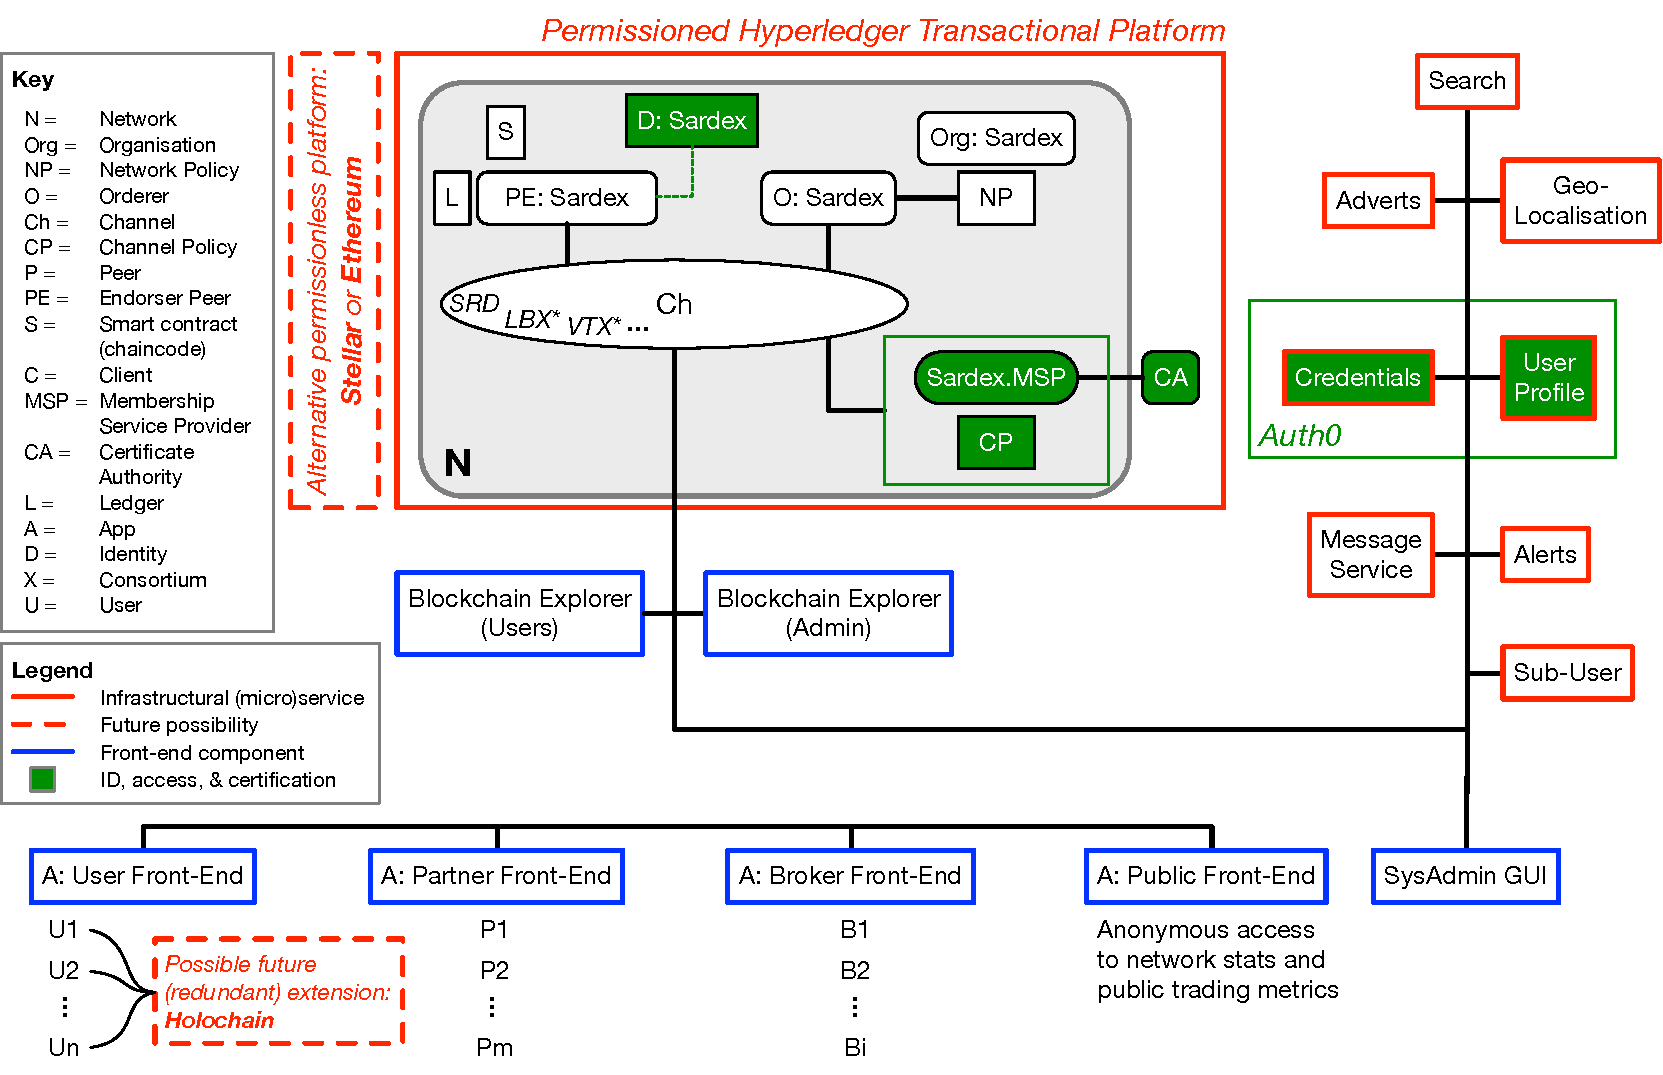
\includegraphics[width=16 cm]{Figures/HL_Architecture}}
\caption{\bf \small High-level Hyperledger-based microservice architecture with possible extensions}
\label{fig:HL_Architecture}
%\vspace{-0.5cm}
\end{figure}

Holochain, on the other hand, could be an interesting extension towards distribution of the blockchain to the end-users, i.e.\ making the end-user terminals (phones) nodes in the blockchain network. This could be interesting for censorship-resistance scenarios, but also for situations where the economy is more informal. For example, in poor neighbourhoods or in contexts where there are migrants, or aid being delivered to migrants. This aspect is farther in the future not only because of the difficulty the realisation of such a financial model would entail but also because the Holochain framework is farther behind in development relative to many others.

\section{INTERLACE Open Shared Architecture}
The final view of the architecture is based on the Corda-Network example,\footnote{\url{https://corda.network/}} which we find deeply interesting and innovative. Its most important aspect, which we plan to emulate, is to separate the Figure \ref{fig:HL_Architecture} view into the three layers shown in Figure \ref{fig:OpenArchitecture} (the orchestration layer is more technically than conceptually relevant so we do not focus on it). This is done not only from the unsurprising functional stack point of view but, more importantly, in terms of the controlling legal entities.

More specifically, the bottom Infrastructure Layer becomes a semi-public, shared, and \emph{neutral} infrastructure as a permissioned blockchain that is a direct extension of the INTERLACE blockchain. Its legal personality could be a foundation, as Corda have done, or similar non-profit entity. However, it will need to be economically self-sustaining; therefore, it will charge for Identity and Notarisation services. The result of this separation is that the bottom, persistence blockchain layer is relatively lightweight -- and therefore of relatively modest operational management requirements. Most the complexity will be housed in the middle layer.

\begin{figure}[h]
\centering
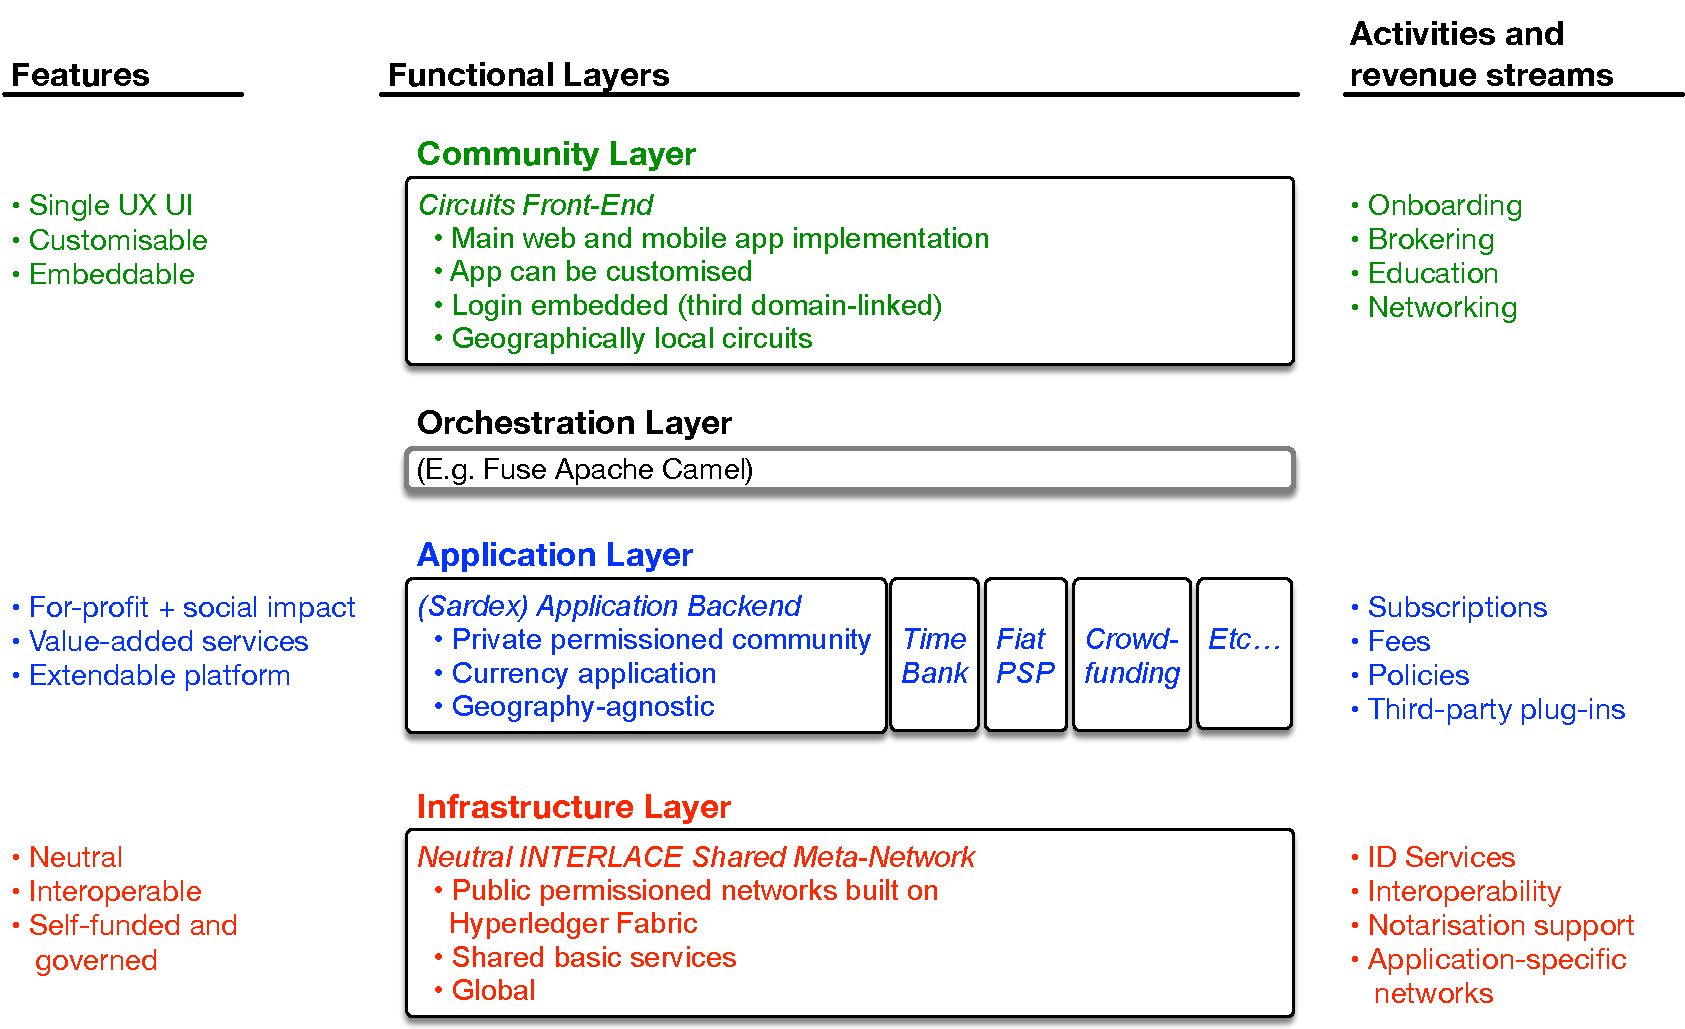
\includegraphics[width=17 cm]{Figures/Open_Shared_Architecture}
\caption{\bf \small Long-term view of the Sardex open shared architecture}
\label{fig:OpenArchitecture}
\end{figure}

The Infrastructure Layer will remain open source. Access will only be given to legal entities, not to natural persons. Finally, this layer will be accessible also to regulators and tax authorities, and will comply with the relevant directives. From the point of view of governance, the Infrastructure Layer will be composed by different kinds of nodes, the first of which will be an Orderer, Identity Certificate Authority, and Notarlsation. But as new nodes join they will take these functions, on rotation, or other functions like Endorser Peer and so forth. These nodes could be run by participating company according to an agreed-upon policy, or by the founding members of the foundation, for example the original members of the INTERLACE project.

The middle, Application Layer is where the proprietary business logic of applications like Sardex will be housed, i.e.\ all the microservices shown in Figure \ref{fig:HL_Architecture}. In the case of the Identity service, it will be split up in order to put the most basic certification aspect in the Infrastructure Layer while the GDPR-relevant user profile data plus other application-specific information will be held in the Application Layer. This layer will also host other applications, shown in the figure as Crowdfunding, normal fiat money Payment Service Providers, and so forth. The implication is that the neutral infrastructure layer will not be limited to credits: because it will not perform deep packet inspection it will mediate whatever the overlying applications will want to transfer. At this layer the architecture can be regarded as centralised since Sardex is the single owner running its proprietary application, even if it might become global.

The third layer is the community layer. This is where localism and the social and cultural dimensions will be represented and protected. This is where both legal entities (mostly but not exclusively SMEs) and natural persons/citizens/consumers will be able to form communities and interact commercially with each other, following the current Sardex model and approach. Each circuit will be run by a `Partner', i.e.\ a for-profit or non-profit company that wishes to set up a Sardex-like circuit in their region.

The next aspect of the architecture to be considered is the interfaces. The interface between the Community and the Application layers will be controlled by the latter through a number of possible GUIs and an appropriate API to support different kinds of Admin access. The managers of the circuits will have a GUI into some of the services of the application, whereas SMEs and natural persons will need to go through their community's GUI/skin. Access will be clocked and charged according to the principles of mutual credit we are currently developing for scalability and that are briefly outlined in deliverable D4.2 \cite{INTERLACE_D42}. For example, the middle-layer application may be partly owned by the circuits which, in turn, may be partly owned by their own users.

The interface between the Application and Infrastructure layers is where the `permissioned' nature of the blockchain is most evident. Depending on the type of company requesting access, different kinds and level of access can be granted. For example, regulators will have a different kind of access from an SME.

\chapter{Conclusion}

\vspace{-1cm}
\begin{center}
Paolo Dini
\end{center}

The question of regulating access is linked to a fundamental aspect of this architecture that has not been mentioned yet. Specifically, it opens the possibility to embed the principles of mutual credit in the infrastructure and the protocols themselves. We make this point in the Conclusion because it highlights the culmination of a journey of increasing self-awareness, self-determination, and appropriation of the technological means that support the financial infrastructure of the Sardex circuit.

The Sardex founders were aware from the beginning that their objective was a radical financial innovation in the service of the local real economy. This can therefore be regarded as a ``political'' project, not in the sense of party politics but in the wider sense of `The Political' as defined for example in the Heteropolitics project:\footnote{\url{https://heteropolitics.net}} \emph{The Political is the deliberate, i.e.\ conscious, choice to form or influence social relations}. The Sardex founders were interested in improving social and economic relations in their territory, but were keenly aware that an explicitly party-political movement would not have been appealing to the great majority of Sardinian SMEs. Thus, they decided to act at the level of a different financial model.

Insofar as a financial model enables and influences economic behaviour and interactions and is encoded in a technology platform, it can be regarded as a form of infrastructure. Because the initial and still-functioning Sardex transactional platform (which INTERLACE aims to replace) is based on a fairly traditional relational database, the original Sardex innovation was ultimately an innovation in \emph{financial architecture} rather than technological architecture. The system architecture that we have presented and discussed in a series of deliverables (D2.1 \cite{INTERLACE_D21}, D2.2 \cite{INTERLACE_D22}, D3.1 \cite{INTERLACE_D31}, D3.2 \cite{INTERLACE_D32}, D4.2 \cite{INTERLACE_D42}) is nothing more than the consequence of this overarching requirement, coupled with the requirement that the system be scalable and sustainable in the long term.

To contextualise the architectural choices around access and mutual credit-specific protocols, it is helpful to view the actions of the Sardex founders and the overarching objectives of the INTERLACE project through the lens of Andrew Feenberg's Critical Theory of Technology (CTT) \cite{Feenberg1999}. Feenberg starts with the assumption that, whether we like it or not, technology embodies our cultural values. As shown in Figure \ref{fig:Feenberg}, Feenberg maps the philosophy of technology field with two axes: in one direction, technology is regarded as either value-neutral or value-laden; in the other direction, it is regarded as either human-controlled or autonomous. The top-left quadrant views technology as autonomous and value-neutral, like Marx's Determinism. The top-right quadrant is populated by people who are optimistic about technology and believe it is neutral. The bottom-left quadrant is populated by Luddites, who fear technology because they regard it as both laden with destructive values and autonomous. INTERLACE belongs firmly in the lower-right quadrant, where our awareness that technology is value-laden together with the belief in our ability to control it leads to a responsible engineering design ethos that can in some sense ``domesticate'' technology by making the technologists accountable to the users of their creations. The importance of bodies like the Internet Governance Forum\footnote{\url{https://www.intgovforum.org/multilingual/content/igf-2018-0}} is ultimately founded on this assumption of responsibility of technology towards society. The foundation or similar body that will eventually control the Infrastructure Layer of the INTERLACE open shared architecture will be organised along similar principles, but with a narrower focus on enabling SMEs through local circuits.

\begin{figure}[h]
\centering
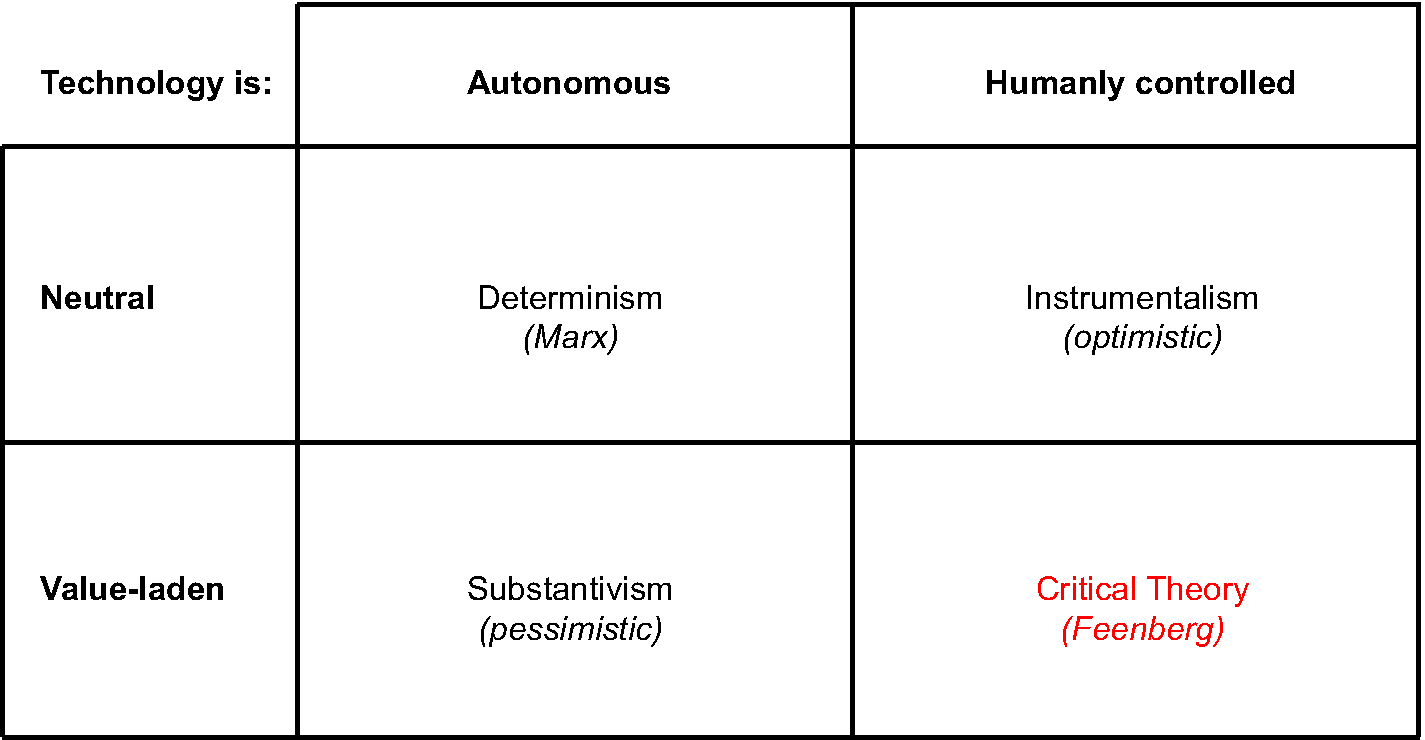
\includegraphics[width=12 cm]{Figures/Feenberg}
\caption{\bf \small The philosophy of technology field according to Feenberg \cite{Feenberg1999}}
\label{fig:Feenberg}
\end{figure}


From this point of view, therefore, the long-term view of the Sardex system is that it will rely on an infrastructure that will enable and support certain kinds of business behaviour while discouraging or making impossible other kinds. Thus, from the CTT viewpoint the Infrastructure Layer is \emph{not} neutral at all, and consciously so. In the previous chapter this layer is characterised as neutral from the point of view of private ownership and competition: it is neutral and open to any legal entities that wish to use it, but the services it will provide are constrained by the non-neutral values that it will embed, namely to support and encourage the real economy and to discourage or block out the financial economy (as it is constituted today).

The clearest examples of how this can be achieved at the level of requirements is to encode the zero-interest and non-convertibility principles into the blockchain protocols/smart contracts that act in this bottom layer. It is not yet clear whether specific access restrictions (to e.g.\ securities traders) should also be enforced, but it may be sufficient (and would be more elegant) simply to disable certain types of financial operations. For example, any mutual credit application that wants to use the blockchain Infrastructure Layer will need to comply with both requirements, but a fiat PSP may need to be able to convert between different currencies. However, even a PSP will not be able to use the blockchain to \emph{store} fiat money or other crypto-currencies, because this blockchain will not be cryptocurrency-based and will not (cannot) be a bank. It can store credits precisely because credits are not regarded, by the banking regulators, to be on the same footing as fiat and, therefore, they are PSD II-exempt.\footnote{\url{https://ec.europa.eu/info/law/payment-services-psd-2-directive-eu-2015-2366_en}}

Similarly, multiple mutual credit system will be able to use the bottom layer, not just Sardex S.p.A., but convertibility between different credit units will not be allowed; this is to prevent the migration of currency exchange speculative practices to the exchange between different credit units. However, if anyone mutual credit application happens to straddle different currency areas, as Sardex is planning to do, then of course an exchange mechanism will be needed given that each credit unit will be pegged 1-1 to its local fiat currency. Another example of a political principle embedded in the protocol, in this case, is the fact that there will be only one exchange rate in both directions between any two currency areas. Finally, these currency exchange rates are an example of the kind of information that will be publicly accessible to anyone, not just the legal entities that have registered to use the permissioned blockchain.

In the long term, we hope that this architecture will enable the scaling of the Sardex mutual credit system to support SME trade worldwide in a way that is transparent and accountable, even if private as concerns business-confidential information and GDPR-regulated personal information; that will be compliant with all banking and PSP regulations; and that will encourage an ecosystem of similarly-minded legal entities in a constructive balance between cooperation and competition in the real economy.



\newpage












\chapter*{References}

\setlength{\parskip}{0.8\baselineskip}
\bibliographystyle{plainurl}
\small
\addcontentsline{toc}{chapter}{References}
\bibliography{Bib/BioComp_References}



\end{document}